\chapter{复杂动力学：链反应、酶与振荡}\label{ch:b3:complex-kinetics}

一烧杯搅拌中的溶液先变为无色，再变为琥珀色，然后变为蓝色，
又恢复无色，并如此持续数分钟；倒入培养皿后，
同一混合物会形成旋转并移动的螺旋图样。当鲍里斯·别洛乌索夫
于 1951 年描述此类反应时，其手稿被退回：审稿人认为，化学体系
不能来回往复，因为它必须朝平衡方向
走下坡路。它确实在走下坡路，只是
并不沿直线走。本章讨论多步机理，其中间体会被再生：
链反应与爆炸、需要碰撞才能单独解离的分子、
酶，以及振荡反应，并介绍
用于跟踪手工混合来不及完成的快速反应的方法。

\begin{recall}
本科一年级分册将反应机理定义为一系列基元反应，
包括决速步、预平衡近似与稳态近似，
以及催化剂。本科二年级分册列出了自由基链的各步，
即链引发、链增长和链终止，并涉及自由基引发剂以及
聚合反应的动力学链长，并拟合了最小二乘直线。
\Cref{ch:b3:rate-theories}给出了过渡态理论与
扩散极限，约为 \qty{e10}{L.mol^{-1}.s^{-1}}。
\end{recall}

\section{链反应}

\begin{definition}[链反应，链载体]\label{def:b3:complex-kinetics:chain}
称\emph{链反应}\index{链反应}为这样一类反应：其中的活性中间体，
即\emph{链载体}\index{链载体}，经
链增长步骤的循环而被再生，使得一次引发事件可以
转化大量反应物分子。
\end{definition}

1906 年，博登斯坦测定了 $\ce{H2 + Br2 -> 2 HBr}$ 的速率，发现了一条
任何单一步骤都无法给出的规律：速率随 $[\ce{Br2}]^{1/2}$ 增大，并随
溴化氢的积累而减小。该机理于 1919 年被写出：
\begin{center}
\begin{tabular}{lll}
引发 & $\ce{Br2 -> 2 Br}$ & $k_1$ \\
链增长 & $\ce{Br + H2 -> HBr + H}$ & $k_2$ \\
链增长 & $\ce{H + Br2 -> HBr + Br}$ & $k_3$ \\
抑制 & $\ce{H + HBr -> H2 + Br}$ & $k_4$ \\
链终止 & $\ce{2 Br -> Br2}$ & $k_{-1}$
\end{tabular}
\end{center}
（在链引发和链终止步骤中，与第三体 M 的碰撞负责输入和带出能量，
此处不予写出）。

\begin{theorem}[氢–溴速率定律]\label{thm:b3:complex-kinetics:hbr}
对 Br 和 H 采用稳态近似，该机理的速率 $v = \frac12\,\dd[\ce{HBr}]/\dd t$
为：
\[
  v = \frac{k[\ce{H2}][\ce{Br2}]^{1/2}}{1 + k'[\ce{HBr}]/[\ce{Br2}]},
  \qquad k = k_2\Bigl(\frac{k_1}{k_{-1}}\Bigr)^{1/2},\ k' = \frac{k_4}{k_3}.
\]
\end{theorem}

\begin{proof}
对 H 的稳态：$k_2[\ce{Br}][\ce{H2}] = k_3[\ce{H}][\ce{Br2}] + k_4[\ce{H}][\ce{HBr}]$。对 Br 的稳态：
$2k_1[\ce{Br2}] - k_2[\ce{Br}][\ce{H2}] + k_3[\ce{H}][\ce{Br2}] + k_4[\ce{H}][\ce{HBr}] - 2k_{-1}[\ce{Br}]^2 = 0$。将两式相加，
链增长项相消，得 $k_1[\ce{Br2}] = k_{-1}[\ce{Br}]^2$，于是 $[\ce{Br}] =
(k_1/k_{-1})^{1/2}[\ce{Br2}]^{1/2}$。再由 $[\ce{H}] = k_2[\ce{Br}][\ce{H2}]/(k_3[\ce{Br2}] + k_4[\ce{HBr}])$，并有
\[
  \frac{\dd[\ce{HBr}]}{\dd t} = k_2[\ce{Br}][\ce{H2}] + k_3[\ce{H}][\ce{Br2}] - k_4[\ce{H}][\ce{HBr}] = 2k_3[\ce{H}][\ce{Br2}]
  = \frac{2k_2[\ce{Br}][\ce{H2}]}{1 + (k_4/k_3)[\ce{HBr}]/[\ce{Br2}]},
\]
利用第一式，代入 $[\ce{Br}]$ 即得结果。
\end{proof}

\begin{omfigure}
\begin{tikzpicture}[font=\small, >=Stealth]
  \node[draw, circle, minimum size=9mm, omDef, thick] (br) at (0,0) {Br};
  \node[draw, circle, minimum size=9mm, omThm, thick] (h) at (4,0) {H};
  \draw[->, thick] (br) to[bend left=35] node[midway, above, align=center] {$+\,\ce{H2}$\\ $\to$ 溴化氢} (h);
  \draw[->, thick] (h) to[bend left=35] node[midway, below, align=center] {$+\,\ce{Br2}$\\ $\to$ 溴化氢} (br);
  \draw[->, thick, black!60] (-2.4,0) -- (br) node[pos=0, left, align=right] {链引发 \\ $\ce{Br2 -> 2 Br}$};
  \draw[->, thick, black!60] (br) -- (0,-2.0) node[below, align=center] {链终止 \\ $\ce{2 Br -> Br2}$};
  \draw[->, thick, black!60, dashed] (h) -- (6.2,-1.2) node[below, align=center] {抑制 \\ $\ce{H + HBr -> H2 + Br}$};
\end{tikzpicture}

{\small 氢–溴链的链增长循环：每循环一次，消耗
一个 \ce{H2} 和一个 \ce{Br2}，生成两个溴化氢，并放出
启动该循环的溴原子。链引发为循环补充载体，链终止则将其除去；
抑制步骤使一个 H 原子变回 Br，
代价是消耗一个已生成的溴化氢。}
\end{omfigure}

\begin{omfigure}
\begin{tikzpicture}
\begin{axis}[name=ca, width=0.47\linewidth, height=5.2cm, xmin=0, xmax=800, ymin=0, ymax=1,
  axis lines=left, xlabel={$t$（约化）}, ylabel={$[\ce{HBr}]/2[\ce{H2}]_0$},
  tick label style={font=\small}, label style={font=\small}]
\addplot[omDef, thick] table[x=t, y expr=\thisrow{HBr}/2] {figdata/out/bachelor-3-chain-kinetics.dat};
\end{axis}
\begin{axis}[at={(ca.east)}, anchor=west, xshift=1.4cm, width=0.47\linewidth, height=5.2cm,
  xmin=0, xmax=60, ymin=0, ymax=2.2, axis lines=left, xlabel={$t$（约化）},
  ylabel={速率 $\times 10^3$}, tick label style={font=\small}, label style={font=\small},
  legend style={font=\scriptsize, draw=none, at={(0.97,0.03)}, anchor=south east},
  legend cell align=left]
\addplot[omDef, thick] table[x=t, y expr=1000*\thisrow{v}] {figdata/out/bachelor-3-chain-kinetics.dat};
\addplot[omThm, thick, dashed] table[x=t, y expr=1000*\thisrow{vss}] {figdata/out/bachelor-3-chain-kinetics.dat};
\legend{完整机理, 稳态速率方程}
\end{axis}
\end{tikzpicture}

{\small 对氢–溴机理逐步积分所得结果（模型
速率常数，约化单位，$k' = 0.1$）：转化率随时间的变化（左），以及
完整机理的速率 $\frac12\dd[\ce{HBr}]/\dd t$ 与稳态速率方程的比较（右）。
经过一段诱导期（期间溴原子逐渐积累）后，两者
吻合程度优于 1\,\%。}
\end{omfigure}

\begin{method}[链式机理的速率方程]\label{met:b3:complex-kinetics:steady-state-chain}
\begin{enumerate}
  \item 对每个链载体写出稳态方程。
  \item 将各式相加：链增长步骤只是把一种载体换成另一种，
        相互抵消后，链引发与链终止相等；
        由此得到载体浓度。
  \item 用其中一种载体的方程表示其余载体。
  \item 由链增长步骤写出某一生成物的生成速率。
\end{enumerate}
\end{method}

每次链引发所对应的链增长循环数，此处为 $v/k_1[\ce{Br2}]$，
即本科二年级分册所说的动力学链长；对氢–溴反应，
它的数量级为 $10^3$ 到 $10^6$，取决于反应条件。产物的抑制作用
解释了为什么速率下降得比反应物被消耗得更快。

\section{链支化与爆炸}

\begin{definition}[链支化、爆炸极限]\label{def:b3:complex-kinetics:branching}
\emph{链支化}\index{链支化}是一步链增长，它生成的链载体
比消耗的更多，例如 $\ce{H + O2 -> OH + O}$，它使一个载体变成两个。
\emph{爆炸极限}\index{爆炸极限}是指
某混合物在给定温度下，使其缓慢反应转为爆炸的
压强。
\end{definition}

\begin{proposition}[支化判据]\label{prop:b3:complex-kinetics:branching}
设载体以速率 $v_i$ 生成，经支化增殖（速率常数为 $f$），
并经终止消失（速率常数为 $g$）：
$\dd n/\dd t = v_i + (f - g)n$。若 $f < g$，则 $n$ 趋于稳定值 $v_i/(g - f)$；若
$f > g$，则 $n$ 指数增长，反应发生爆炸。
\end{proposition}

\begin{proof}
线性方程的解为 $n(t) = \frac{v_i}{g - f}\bigl(1 - \eu^{-(g - f)t}\bigr)$，
它趋于 $v_i/(g - f)$（设 $g > f$）；当 $f > g$ 时指数为正，$n$
按 $\eu^{(f - g)t}$ 无界增长（直至反应物耗尽）。
\end{proof}

对于几百摄氏度下的氢–氧混合物，$f$ 随
压强增大而增大（与 $[\ce{O2}]$ 成正比），器壁上的终止
在低压下很快（自由基很容易扩散到器壁），而
三体碰撞终止（$\ce{H + O2 + M -> HO2 + M}$）
随压强的平方增长。支化在由器壁决定的第一极限与
由三体终止决定的第二极限之间占优；更高压强下又出现第三极限，
即释放的热量不能再散失之处。最后一种是
热爆炸，它由速率随温度的指数增长所驱动，而非由支化所驱动；
大多数工业爆炸都属于
此类。

\section{单分子反应}

像环丙烷这样的分子可单独发生异构化，在常压下遵循一级动力学；
然而在低压下速率常数会下降。所需能量来自
分子间的碰撞。

\begin{definition}[林德曼机理、衰减区]\label{def:b3:complex-kinetics:lindemann}
单分子反应的\emph{林德曼机理}\index{林德曼机理}是如下
过程：$\mathrm{A + M \rightleftharpoons A^* + M}$（$k_1$、$k_{-1}$），由与任一分子 M 碰撞实现活化和失活，
随后为 $\mathrm{A^* \to P}$（$k_2$）。
\emph{衰减区}\index{衰减区}是指压强的一个范围，在此范围内
观测到的一级速率常数由其高压值起
逐渐下降，趋向二级行为。
\end{definition}

\begin{theorem}[林德曼速率常数]\label{thm:b3:complex-kinetics:lindemann}
对 $\mathrm{A^*}$ 采用稳态近似，有 $v = k_{\mathrm{uni}}[\mathrm A]$，其中
\[
  k_{\mathrm{uni}} = \frac{k_1k_2[\mathrm M]}{k_{-1}[\mathrm M] + k_2},
\]
它在高压下趋于 $k_\infty = k_1k_2/k_{-1}$（一级），在
低压下趋于 $k_1[\mathrm M]$（二级）；其值为 $k_\infty/2$，此时 $[\mathrm M]_{1/2} = k_2/k_{-1}$。
\end{theorem}

\begin{proof}
令 $\dd[\mathrm{A^*}]/\dd t = k_1[\mathrm A][\mathrm M] - k_{-1}[\mathrm{A^*}][\mathrm M] - k_2[\mathrm{A^*}] = 0$，得 $[\mathrm{A^*}] =
k_1[\mathrm A][\mathrm M]/(k_{-1}[\mathrm M] + k_2)$，且 $v = k_2[\mathrm{A^*}]$。若 $k_{-1}[\mathrm M] \gg k_2$，则失活
快于反应，$\mathrm{A^*}$ 处于预平衡，$k_{\mathrm{uni}} \to k_1k_2/k_{-1}$。若 $k_{-1}[\mathrm M]
\ll k_2$，则每个活化分子都参与反应，活化成为决速步：
$k_{\mathrm{uni}} \to k_1[\mathrm M]$。
\end{proof}

\begin{omfigure}
\begin{tikzpicture}
\begin{axis}[width=0.66\linewidth, height=5.4cm, xmode=log, ymode=log, xmin=1e-10, xmax=1e-2,
  ymin=1e-8, ymax=4e-3, axis lines=left, xlabel={$[\mathrm M]$ / \unit{mol.L^{-1}}},
  ylabel={$k_{\mathrm{uni}}$ / \unit{s^{-1}}}, tick label style={font=\small}, label style={font=\small}]
\addplot[black!40, dashed] table[x=M, y=low] {figdata/out/bachelor-3-lindemann.dat};
\addplot[black!40, dashed] table[x=M, y=high] {figdata/out/bachelor-3-lindemann.dat};
\addplot[omDef, very thick] table[x=M, y=k] {figdata/out/bachelor-3-lindemann.dat};
\node[font=\scriptsize, anchor=south, rotate=39] at (axis cs:4e-9,2.5e-5) {$k_1[\mathrm M]$};
\node[font=\scriptsize, anchor=south] at (axis cs:3e-4,1e-3) {$k_\infty$};
\draw[black!50, densely dotted] (axis cs:1e-6,1e-8) -- (axis cs:1e-6,5e-4);
\node[font=\scriptsize, anchor=north west] at (axis cs:1.2e-6,2e-7) {$[\mathrm M]_{1/2}$};
\end{axis}
\end{tikzpicture}

{\small 林德曼衰减曲线（模型常数）：高压下为一级，
极限速率常数为 $k_\infty$；低压下为二级（$k_1[\mathrm M]$）；
$k_\infty$ 的一半出现在 $[\mathrm M]_{1/2} = k_2/k_{-1}$ 处。实际的衰减曲线较宽：高能分子的
速率常数 $k_2$ 随其能量增大而增大。}
\end{omfigure}

\section{酶动力学}

\begin{definition}[酶、活性位点、酶–底物复合物]\label{def:b3:complex-kinetics:enzyme}
\emph{酶}\index{酶}是一种生物催化剂，几乎总是蛋白质，
能加速其底物的某一特定反应。\emph{活性位点}\index{活性位点}是酶的口袋状区域，
底物在其中结合并发生反应；结合后的物种
称为\emph{酶–底物复合物}\index{酶–底物复合物}，
记作 ES。
\end{definition}

\begin{definition}[米氏常数、最大速率、催化常数与专一性常数]\label{def:b3:complex-kinetics:michaelis}
对于反应机理 $\mathrm{E + S \rightleftharpoons ES \to E + P}$（$k_1$、$k_{-1}$、$k_2$），
在总酶浓度 $[\mathrm E]_0$ 下，\emph{催化常数}\index{催化常数}为 $k_{\mathrm{cat}} = k_2$，
\emph{最大速率}\index{最大速率}为 $V_{\max} = k_{\mathrm{cat}}[\mathrm E]_0$，\emph{米氏常数}
\index{米氏常数}为 $K_M = (k_{-1} + k_2)/k_1$，\emph{专一性常数}
\index{专一性常数}为 $k_{\mathrm{cat}}/K_M$。
\end{definition}

\begin{theorem}[米氏方程]\label{thm:b3:complex-kinetics:michaelis-menten}
当 $[\mathrm S] \gg [\mathrm E]_0$ 且 ES 处于稳态时，
产物的初始生成速率为
\[
  v = \frac{V_{\max}[\mathrm S]}{K_M + [\mathrm S]} .
\]
此式称为\emph{米氏方程}\index{米氏方程}。
\end{theorem}

\begin{proof}
稳态条件为 $k_1[\mathrm E][\mathrm S] = (k_{-1} + k_2)[\mathrm{ES}]$，且 $[\mathrm E] = [\mathrm E]_0 - [\mathrm{ES}]$，
（游离底物几乎即为全部底物，因为 $[\mathrm S] \gg [\mathrm E]_0$）。因此 $[\mathrm{ES}]
= [\mathrm E]_0[\mathrm S]/(K_M + [\mathrm S])$，则 $v = k_2[\mathrm{ES}]$。
\end{proof}

\begin{remark}
米氏（1913）改为假设 E、S 与 ES 之间快速
建立预平衡，此时同一方程仍成立，只需把 $K_M$ 换为解离常数 $k_{-1}/k_1$，
即 $K_M$ 在 $k_2 \ll k_{-1}$ 时的极限。催化常数即
生物化学家所称的酶的转化数，即饱和时
一个活性位点每秒转化的底物分子数。
\end{remark}

当 $[\mathrm S] = K_M$ 时速率为 $V_{\max}/2$；当 $[\mathrm S] \ll K_M$ 时速率为 $(k_{\mathrm{cat}}/K_M)[\mathrm E]_0[\mathrm S]$：
专一性常数即游离酶与其底物的二级速率常数，
它不可能超过二者相遇的速率，即
\cref{ch:b3:rate-theories}中的扩散极限。少数酶接近该极限；
“平均”的酶，在对数千种酶的调查中，$k_{\mathrm{cat}}/K_M$ 约为
$10^5$~\unit{L.mol^{-1}.s^{-1}}，比其低约四个数量级。

\begin{proposition}[林韦弗–伯克形式]\label{prop:b3:complex-kinetics:lineweaver}
米氏方程等价于
\[
  \frac1v = \frac{1}{V_{\max}} + \frac{K_M}{V_{\max}}\,\frac{1}{[\mathrm S]},
\]
即以 $1/v$ 对 $1/[\mathrm S]$ 作图的直线，截距为 $1/V_{\max}$，斜率为 $K_M/V_{\max}$，
另一截距为 $-1/K_M$，位于 $1/[\mathrm S]$ 轴上。
\end{proposition}

\begin{proof}
取倒数得 $1/v = (K_M + [\mathrm S])/(V_{\max}[\mathrm S])$。当 $1/v = 0$ 时，$1/[\mathrm S] = -1/K_M$。
\end{proof}

\begin{method}[用非线性最小二乘法求 $K_M$ 与 $V_{\max}$]\label{met:b3:complex-kinetics:mm-fit}
\begin{enumerate}
  \item 测定初始速率，底物浓度分布于约 $K_M/5$ 至 $10K_M$ 之间
        的范围内。
  \item 直接拟合 $v = V_{\max}[\mathrm S]/(K_M + [\mathrm S])$，通过最小化 $\sum(v_i - v(\mathrm S_i))^2$（迭代进行，
        以林韦弗–伯克直线的值为初值）；标准误差
        由残差及 $v$ 对每个参数的
        灵敏度求得。
  \item 林韦弗–伯克图仅用于观察规律：对较小的速率取倒数
        会放大其误差，因此对 $1/v$ 所作的最小二乘直线
        主要受精度最差的数据点支配，其参数
        存在偏倚。
\end{enumerate}
\end{method}

\begin{definition}[抑制]\label{def:b3:complex-kinetics:inhibition}
抑制剂 I 与酶可逆结合。在\emph{竞争性
抑制}\index{竞争性抑制}中，它只与游离酶结合，且结合于
活性位点，其\emph{抑制常数}\index{抑制常数} $K_i$
（即 EI 的解离常数）；在\emph{反竞争性抑制}\index{反竞争性抑制}中，
它只与 ES 结合，其常数为 $K_i'$；在\emph{混合型
抑制}\index{混合型抑制}中，它与二者均结合。
\end{definition}

\begin{proposition}[抑制作用下的速率规律]\label{prop:b3:complex-kinetics:inhibition-laws}
记 $\alpha = 1 + [\mathrm I]/K_i$，$\alpha' = 1 + [\mathrm I]/K_i'$，则速率仍保持
米氏形式 $v = V^{\mathrm{app}}[\mathrm S]/(K_M^{\mathrm{app}} + [\mathrm S])$，其中竞争性：
$K_M^{\mathrm{app}} = \alpha K_M$，$V^{\mathrm{app}} = V_{\max}$；反竞争性：$K_M^{\mathrm{app}} = K_M/\alpha'$，$V^{\mathrm{app}} =
V_{\max}/\alpha'$；混合型：$K_M^{\mathrm{app}} = \alpha K_M/\alpha'$，$V^{\mathrm{app}} = V_{\max}/\alpha'$。
\end{proposition}

\begin{proof}
混合型情形（其余两种为其极限 $K_i' \to \infty$ 与 $K_i \to \infty$）：酶
分配于 E、EI、ES 与 ESI 之间，其中 $[\mathrm{EI}] = [\mathrm E][\mathrm I]/K_i$，$[\mathrm{ESI}] = [\mathrm{ES}][\mathrm I]/K_i'$，
且稳态条件为 $[\mathrm E][\mathrm S] = K_M[\mathrm{ES}]$。于是 $[\mathrm E]_0 = [\mathrm E]\alpha + [\mathrm{ES}]\alpha' =
[\mathrm{ES}](\alpha K_M/[\mathrm S] + \alpha')$，则 $v = k_2[\mathrm{ES}] = V_{\max}[\mathrm S]/(\alpha K_M + \alpha'[\mathrm S])$；以 $\alpha'$ 同除分子与分母，
即得所述形式。
\end{proof}

\begin{method}[判别抑制的类型]\label{met:b3:complex-kinetics:inhibition-type}
\begin{enumerate}
  \item 在几种抑制剂浓度下测定 $v([\mathrm S])$，并作出
        林韦弗–伯克直线。
  \item 直线交于 $1/v$ 轴上（$V_{\max}$ 相同）：竞争性；大量过量的
        底物可克服抑制剂的作用。
  \item 直线平行（斜率 $K_M/V_{\max}$ 不变）：反竞争性。
  \item 直线交于 $1/v$ 轴左侧：混合型。
  \item 求得 $K_i$ 时，对表观常数作关于 $[\mathrm I]$ 的拟合：对竞争性抑制剂，
        $K_M^{\mathrm{app}} = K_M + (K_M/K_i)[\mathrm I]$，为一条直线。
\end{enumerate}
\end{method}

\begin{omfigure}
\begin{tikzpicture}
\begin{axis}[name=mv, width=0.47\linewidth, height=5.4cm, xmin=0, xmax=8, ymin=0, ymax=0.55,
  axis lines=left, xlabel={$[\mathrm S]$ / mM}, ylabel={$v$ / \unit{\micro M.s^{-1}}},
  tick label style={font=\small}, label style={font=\small},
  legend style={font=\scriptsize, draw=none, fill=white, fill opacity=0.85, text opacity=1,
  at={(0.97,0.03)}, anchor=south east}, legend cell align=left]
\addplot[black, thick] table[x=S, y=none] {figdata/out/bachelor-3-michaelis-menten-model.dat};
\addplot[omDef, thick] table[x=S, y=comp] {figdata/out/bachelor-3-michaelis-menten-model.dat};
\addplot[omThm, thick] table[x=S, y=uncomp] {figdata/out/bachelor-3-michaelis-menten-model.dat};
\draw[black!40, densely dotted] (axis cs:0,0.25) -- (axis cs:0.8,0.25) -- (axis cs:0.8,0);
\node[font=\scriptsize, anchor=north west] at (axis cs:0.85,0.12) {$K_M$};
\legend{无抑制剂, 竞争性, 反竞争性}
\end{axis}
\begin{axis}[at={(mv.east)}, anchor=west, xshift=1.5cm, width=0.47\linewidth, height=5.4cm,
  xmin=-2.5, xmax=3.5, ymin=0, ymax=12, axis x line=middle, axis y line=middle,
  tick label style={font=\small}, xtick={-2,-1,1,2,3}]
\node[font=\small, anchor=south east] at (axis cs:3.5,0.3) {$1/[\mathrm S]$};
\node[font=\small, anchor=north west] at (axis cs:0.12,12) {$1/v$};
\addplot[black, thick, domain=-1.25:3.5] {1.6*x + 2};
\addplot[omDef, thick, domain=-0.4167:3.5] {4.8*x + 2};
\addplot[omThm, thick, domain=-2.5:3.5] {1.6*x + 4};
\end{axis}
\end{tikzpicture}

{\small 米氏动力学，取 $K_M = \qty{0.80}{mM}$ 和 $V_{\max} = \qty{0.50}{\micro M.s^{-1}}$
（模型）：无抑制剂（黑色），竞争性抑制剂在 $[\mathrm I] = 2K_i$ 时（蓝色，
$K_M$ 增至三倍，$V_{\max}$ 不变）；反竞争性抑制剂在 $[\mathrm I] = K_i'$ 时（红色，$K_M$ 和
$V_{\max}$ 均减半）。右图为林韦弗–伯克直线，竞争性抑制的直线
与无抑制的直线相交于 $1/v$ 轴，反竞争性抑制的直线与之平行
（$1/[\mathrm S]$ 的单位为 \unit{mM^{-1}}，$1/v$ 的单位为 \unit{s.\micro M^{-1}}）。}
\end{omfigure}

\section{自催化、振荡与快速反应}

\begin{definition}[自催化反应]\label{def:b3:complex-kinetics:autocatalysis}
称\emph{自催化反应}\index{自催化反应}为这样一种反应：其中某一生成物
催化其自身的生成，如 $\mathrm{A + X \to 2\,X}$。
\end{definition}

\begin{proposition}[逻辑斯谛定律]\label{prop:b3:complex-kinetics:logistic}
对 $\mathrm{A + X \to 2\,X}$，设速率常数为 $k$，初始浓度分别为 $a_0$ 和 $x_0$，
记 $N = a_0 + x_0$，
\[
  x(t) = \frac{N}{1 + (N/x_0 - 1)\eu^{-kNt}},
\]
这是一条 S 形曲线，在 $t_{1/2} = \ln(N/x_0 - 1)/kN$ 时达到终值的一半。
\end{proposition}

\begin{proof}
$\dd x/\dd t = kx(N - x)$，因 $a = N - x$。分离变量，$\frac{\dd x}{x(N - x)} = \frac1N\bigl(\frac1x + \frac{1}{N - x}\bigr)\dd x
= k\,\dd t$，于是 $\ln\frac{x}{N - x} = kNt + \ln\frac{x_0}{N - x_0}$，整理即得所述形式；
$x = N/2$，此即 $(N/x_0 - 1)\eu^{-kNt} = 1$。
\end{proof}

\begin{definition}[振荡反应、极限环]\label{def:b3:complex-kinetics:oscillating}
称\emph{振荡反应}\index{振荡反应}为这样一种反应：其中
中间体的浓度周期性地升降，而总反应
趋向平衡。称\emph{极限环}\index{极限环}为
浓度空间中的一条闭合轨迹，其附近的
轨迹都向它收敛，从而振荡的振幅与
出发点无关。
\end{definition}

\begin{theorem}[洛特卡–沃尔泰拉模型]\label{thm:b3:complex-kinetics:lotka-volterra}
对自催化方案 $\mathrm{A + X \to 2\,X}$、$\mathrm{X + Y \to 2\,Y}$、$\mathrm{Y \to B}$，设 A 保持
不变，浓度满足 $\dot x = x(a - by)$、$\dot y = y(dx - c)$，其中常数均为正，
并考虑下述量
\[
  V = dx - c\ln x + by - a\ln y
\]
沿每条轨迹为常数：轨迹是绕稳态
$(c/d, a/b)$ 的闭曲线，浓度振荡，其振幅由
出发点决定。
\end{theorem}

\begin{proof}
$\dot V = (d - c/x)\dot x + (b - a/y)\dot y = (dx - c)(a - by) + (by - a)(dx - c) = 0$。$V$ 是两个
凸函数之和，在 $(c/d, a/b)$ 处有唯一极小值，故其水平集
为绕该点的闭曲线；轨迹停留在其中一条上，
且速度在别处从不为零，因而周期性地绕该点运行。
\end{proof}

洛特卡–沃尔泰拉振荡是脆弱的：每个出发点都给出
各自的轨道，任何扰动都会使系统转到另一条轨道上。实际化学
振子具有极限环，这需要一种能使
稳态失稳的非线性机制。

\begin{proposition}[布鲁塞尔振子的失稳]\label{prop:b3:complex-kinetics:hopf}
该模型 $\dot X = A - (B + 1)X + X^2Y$、$\dot Y = BX - X^2Y$（约化浓度，
$A$ 和 $B$ 保持不变），具有唯一稳态 $(A, B/A)$，该稳态
在 $B < 1 + A^2$ 时稳定，在 $B > 1 + A^2$ 时不稳定；此时系统
趋于一个极限环。
\end{proposition}

\begin{proof}
令两导数为零：由 $BX = X^2Y$ 得 $XY = B$，进而 $A - X = 0$。
在 $(A, B/A)$ 处的雅可比矩阵为
\[
  \begin{pmatrix} -(B + 1) + 2XY & X^2 \\ B - 2XY & -X^2 \end{pmatrix}
  = \begin{pmatrix} B - 1 & A^2 \\ -B & -A^2 \end{pmatrix},
\]
其迹为 $B - 1 - A^2$，行列式为 $A^2 > 0$。小扰动按
$\eu^{\lambda t}$ 演化，其中 $\lambda$ 为本征值，其积为行列式（正），
和为迹：迹为负时两者实部均为负，
迹为正时实部均为正。对 $B > 1 + A^2$ 的极限环存在性
（轨迹限于有界区域内）在本阶段
不加证明地承认。
\end{proof}

\begin{method}[稳态的线性稳定性]\label{met:b3:complex-kinetics:stability}
\begin{enumerate}
  \item 令所有时间导数为零，求出稳态。
  \item 计算该点处速率对各变量偏导数构成的雅可比矩阵。
  \item 对两个变量：若迹为负且行列式为正，则稳态稳定；
        若稳态不稳定且本征值为复数
        （$\mathrm{tr}^2 < 4\det$）则产生增长的振荡，即可能的极限环。
\end{enumerate}
\end{method}

\begin{omfigure}
\begin{tikzpicture}
\begin{axis}[name=bs, width=0.62\linewidth, height=4.6cm, xmin=0, xmax=40, ymin=0, ymax=5.2,
  axis lines=left, xlabel={$t$（约化）}, ylabel={浓度},
  tick label style={font=\small}, label style={font=\small},
  legend style={font=\scriptsize, draw=none, at={(1.03,0.98)}, anchor=north west}]
\addplot[omDef, thick] table[x=t, y=X] {figdata/out/bachelor-3-oscillations-series.dat};
\addplot[omThm, thick] table[x=t, y=Y] {figdata/out/bachelor-3-oscillations-series.dat};
\legend{$X$, $Y$}
\end{axis}
\begin{axis}[name=ph, at={(bs.below south west)}, anchor=north west, yshift=-0.6cm,
  width=0.42\linewidth, height=5.0cm, xmin=0, xmax=4.8, ymin=0, ymax=5.6, axis lines=left,
  xlabel={$X$}, ylabel={$Y$}, tick label style={font=\small}, label style={font=\small},
  title={\small 布鲁塞尔振子}]
\addplot[omDef, thin] table[x=X, y=Y] {figdata/out/bachelor-3-oscillations-inner.dat};
\addplot[omThm, thin] table[x=X, y=Y] {figdata/out/bachelor-3-oscillations-outer.dat};
\addplot[only marks, mark=*, mark size=1.5pt] coordinates {(1,3)};
\end{axis}
\begin{axis}[at={(ph.east)}, anchor=west, xshift=1.3cm, width=0.42\linewidth, height=5.0cm,
  xmin=0, xmax=3.2, ymin=0, ymax=3.2, axis lines=left, xlabel={$x$}, ylabel={$y$},
  tick label style={font=\small}, label style={font=\small}, title={\small 洛特卡–沃尔泰拉}]
\addplot[black!70, thick] table[x=x, y=y] {figdata/out/bachelor-3-oscillations-lv1.dat};
\addplot[omDef, thick] table[x=x, y=y] {figdata/out/bachelor-3-oscillations-lv2.dat};
\addplot[omThm, thick] table[x=x, y=y] {figdata/out/bachelor-3-oscillations-lv3.dat};
\addplot[only marks, mark=*, mark size=1.5pt] coordinates {(1,1)};
\end{axis}
\end{tikzpicture}

{\small 上图：布鲁塞尔模型（$A = 1$，$B = 3 > 1 + A^2$）进入持续振荡，
周期为 7.2（约化时间）。下左：两条轨迹，一条起点靠近不稳定稳态（圆点），
另一条起点远离，二者都盘绕到同一极限环上。下右：
洛特卡–沃尔泰拉轨道，各由其起点确定，
绕稳态（圆点）运行。}
\end{omfigure}

别洛索夫–扎博廷斯基反应是丙二酸被溴酸盐氧化的反应，
催化剂为铈或亚铁灵指示剂，它经历这样一个循环：自催化生成
\ce{HBrO2} 的过程在溴离子降到
阈值以下时开启，氧化催化剂（使颜色改变），并在
氧化后的催化剂再生溴离子时被关闭。若不搅拌、置于薄层中，
振荡便以波的形式传播。

\begin{omfigure}
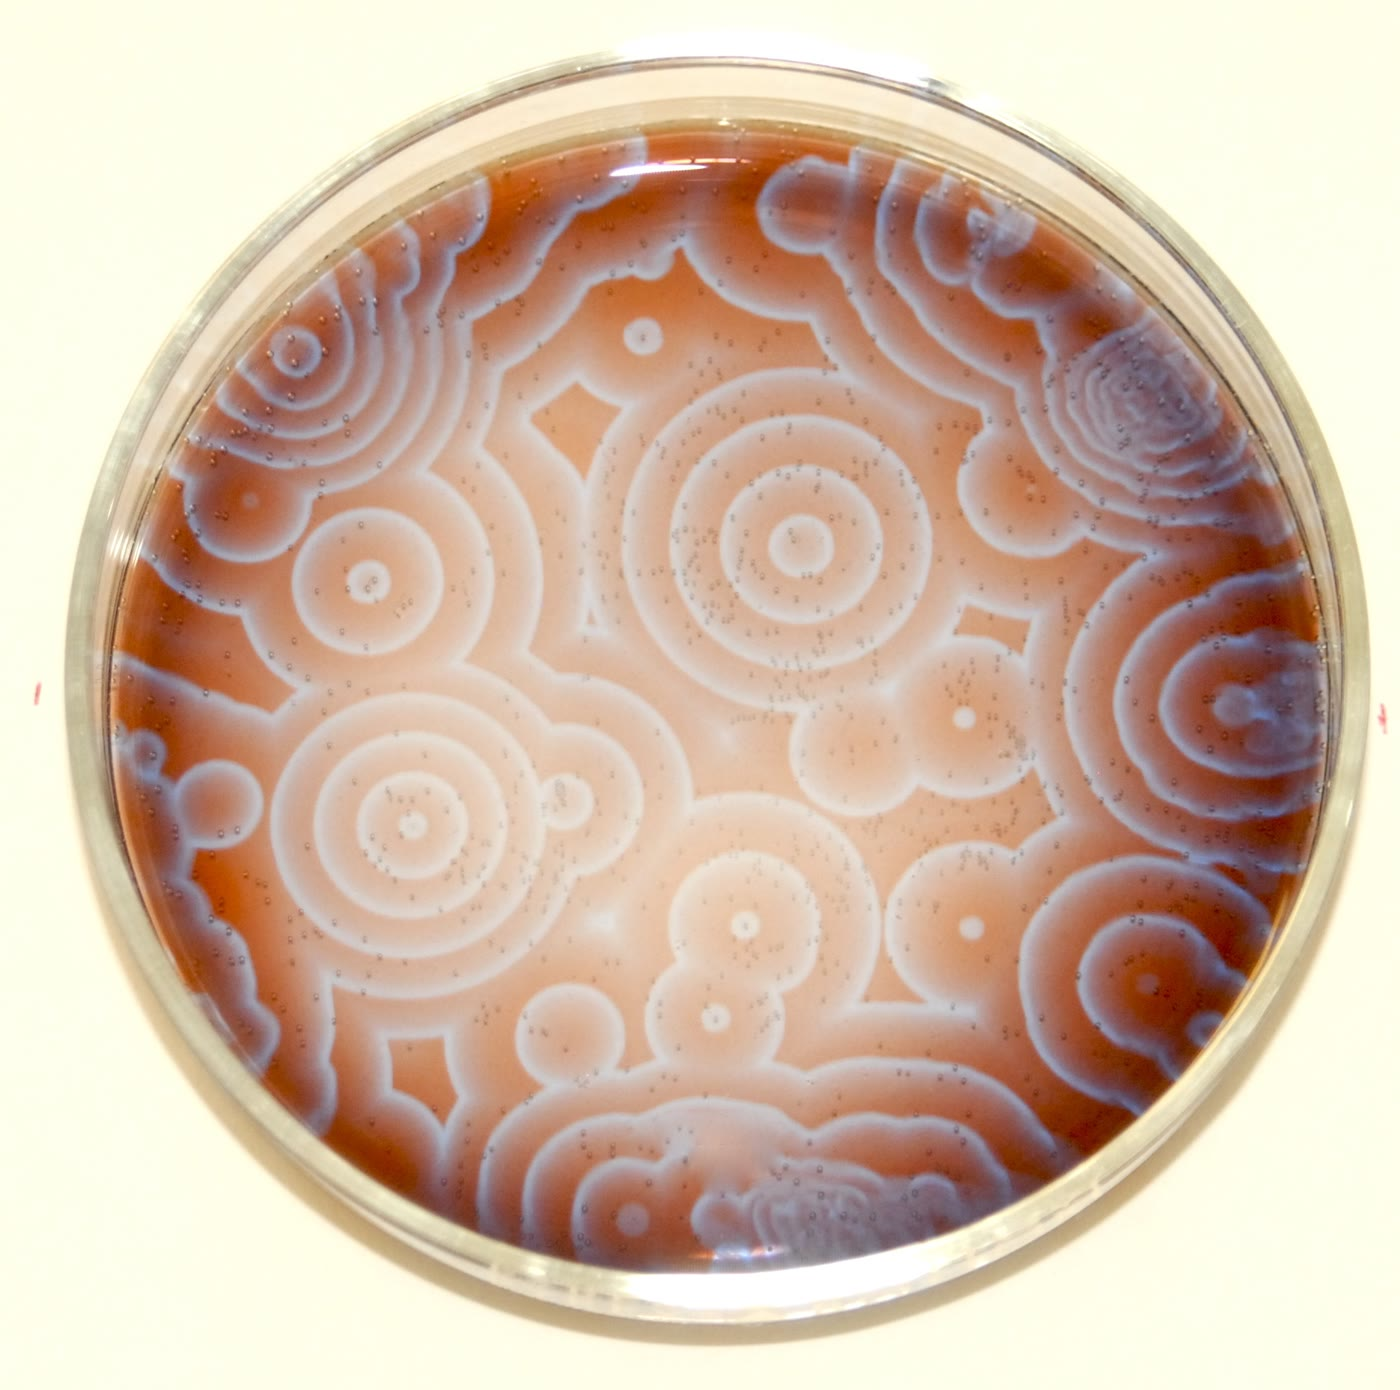
\includegraphics[width=0.48\linewidth]{images/book4/bz-reaction.jpg}

{\small 薄层溶液中别洛索夫–扎博廷斯基反应的螺旋波：
每一条蓝色波前都是催化剂的氧化波，它
进入被还原的（红色）介质，且不会重新进入
刚离开的区域。}
\end{omfigure}

\begin{definition}[弛豫法，化学弛豫时间]\label{def:b3:complex-kinetics:relaxation}
\emph{弛豫法}\index{弛豫法}使处于平衡的体系
突然受到扰动（如温度、压强或电场的跃变），
并跟踪其回到新平衡的过程。对于小扰动，
偏离量按指数规律衰减，衰减的特征量为
\emph{化学弛豫时间}\index{化学弛豫时间} $\tau$。
\end{definition}

\begin{proposition}[缔合反应的弛豫时间]\label{prop:b3:complex-kinetics:relaxation-time}
对于 $\mathrm{A + B \rightleftharpoons C}$（$k_1$，$k_{-1}$），小扰动之后，
\[
  \frac1\tau = k_1([\mathrm A]_e + [\mathrm B]_e) + k_{-1} .
\]
\end{proposition}

\begin{proof}
设 $[\mathrm C] = [\mathrm C]_e + x$，$[\mathrm A] = [\mathrm A]_e - x$，$[\mathrm B] = [\mathrm B]_e - x$。则 $\dot x =
k_1([\mathrm A]_e - x)([\mathrm B]_e - x) - k_{-1}([\mathrm C]_e + x)$；不含 $x$ 的项在平衡时相互抵消，
略去 $x^2$ 项，得 $\dot x = -[k_1([\mathrm A]_e + [\mathrm B]_e) + k_{-1}]x$。
\end{proof}

在若干浓度下测量 $\tau$，得到 $1/\tau$ 对 $[\mathrm A]_e +
[\mathrm B]_e$ 的直线，其斜率为 $k_1$，截距为 $k_{-1}$：这两个常数都来自
体系偏离平衡不超过百分之几的实验。曼弗雷德·艾根
以此方法测定了溶液中最快的一些反应，
其中包括 \ce{H3O+} 被 \ce{OH-} 中和的反应。

\begin{omfigure}
\begin{tikzpicture}
\begin{axis}[width=0.62\linewidth, height=5.0cm, xmin=0, xmax=780, ymin=0, ymax=1.05,
  axis lines=left, xlabel={$t$ / \unit{\micro s}}, ylabel={$([\mathrm C] - [\mathrm C]_e)/([\mathrm C]_0 - [\mathrm C]_e)$},
  tick label style={font=\small}, label style={font=\small},
  legend style={font=\scriptsize, draw=none, at={(0.97,0.97)}, anchor=north east},
  legend cell align=left]
\addplot[omDef, very thick] table[x=t_us, y=dC] {figdata/out/bachelor-3-chemical-relaxation.dat};
\addplot[omThm, thick, dashed] table[x=t_us, y=exp] {figdata/out/bachelor-3-chemical-relaxation.dat};
\legend{完整速率方程，{$\eu^{-t/\tau}$，$\tau = \qty{156}{\micro s}$}}
\draw[black!40, densely dotted] (axis cs:156,0) -- (axis cs:156,0.368) -- (axis cs:0,0.368);
\end{axis}
\end{tikzpicture}

{\small $\mathrm{A + B \rightleftharpoons C}$ 的弛豫过程，由温度跃变引起，使其平衡常数降低了 5\,\%
（模型取 $k_1 = \qty{1.0e8}{L.mol^{-1}.s^{-1}}$，$k_{-1} = \qty{1.0e3}{s^{-1}}$，A 和 B 的
初始浓度均为 \qty{1.0e-4}{mol/L}）：完整速率方程与
满足 $1/\tau = k_1([\mathrm A]_e + [\mathrm B]_e) + k_{-1}$ 的指数曲线相互重合。}
\end{omfigure}

\begin{definition}[停流法，闪光光解]\label{def:b3:complex-kinetics:fast}
\emph{停流法}\index{停流法}在约一毫秒内将两份反应物溶液
经混合器推入观测池中混合，
然后停止流动，并记录吸光度或荧光。
\emph{闪光光解}\index{闪光光解}借助短促而强烈的光脉冲
产生活性物种，并用第二束延迟的
光束跟踪其反应。
\end{definition}

\begin{omfigure}
\begin{tikzpicture}[font=\small, >=Stealth]
  % two drive syringes
  \foreach \y/\lab in {1.1/A, -0.1/B}{
    \draw[thick] (0,\y) rectangle (2.2,\y+0.6);
    \fill[omDef!25] (0.6,\y+0.05) rectangle (2.15,\y+0.55);
    \draw[thick] (0.6,\y) -- (0.6,\y+0.6);
    \draw[thick] (-0.6,\y+0.3) -- (0.6,\y+0.3);
    \node at (1.4,\y+0.3) {\lab};
    \draw[thick] (2.2,\y+0.3) -- (2.8,\y+0.3);}
  \draw[thick] (2.8,1.4) -- (3.2,0.8) (2.8,0.2) -- (3.2,0.8);
  \node[draw, thick, circle, minimum size=5mm, fill=white] (mx) at (3.4,0.8) {};
  \node[font=\scriptsize, anchor=north] at (3.4,0.5) {混合器};
  \draw[thick] (mx.east) -- (4.4,0.8);
  \draw[thick, fill=omThm!15] (4.4,0.55) rectangle (5.4,1.05);
  \node[font=\scriptsize, anchor=north west, align=left] at (5.0,0.5) {观测 \\池};
  \draw[->, omThm, thick] (4.9,2.0) -- (4.9,1.1) node[pos=0, above, font=\scriptsize] {光};
  \draw[->, omThm, thick] (4.9,0.5) -- (4.9,-0.4) node[below, font=\scriptsize] {检测器};
  \draw[thick] (5.4,0.8) -- (6.2,0.8);
  \draw[thick] (6.2,0.5) rectangle (7.6,1.1);
  \draw[thick] (7.0,0.5) -- (7.0,1.1);
  \draw[thick] (7.0,0.8) -- (7.9,0.8);
  \draw[thick] (7.9,0.4) -- (7.9,1.2);
  \node[font=\scriptsize, anchor=south] at (6.9,1.15) {停止注射器};
  \draw[->, black!60] (-1.2,1.4) -- (-0.7,1.4) node[pos=0, left, font=\scriptsize] {驱动};
  \draw[->, black!60] (-1.2,0.2) -- (-0.7,0.2);
\end{tikzpicture}

{\small 停流装置示意图。驱动装置推动两个注射器；两种溶液
在混合器中相遇，并在约一毫秒内充满观测池；
停止注射器的活塞撞上挡块，流动停止，
检测器记录刚混合的溶液的反应。}
\end{omfigure}

\begin{omfigure}
\begin{tikzpicture}
\begin{axis}[width=0.62\linewidth, height=5.0cm, xmin=0, xmax=20, ymin=0, ymax=5.5,
  axis lines=left, xlabel={$t$ / ms}, ylabel={$[\mathrm P_1]$ / \unit{\micro M}},
  tick label style={font=\small}, label style={font=\small}]
\addplot[omDef, very thick] table[x=t_ms, y=P_uM] {figdata/out/bachelor-3-michaelis-menten-burst.dat};
\addplot[black!45, dashed, domain=0:20] {1.28 + 0.2*x};
\draw[->, black!60] (axis cs:4.5,0.7) -- (axis cs:0.25,1.24);
\node[font=\scriptsize, anchor=west] at (axis cs:4.5,0.7) {爆发幅度，\qty{1.28}{\micro M}};
\end{axis}
\end{tikzpicture}

{\small 停流法测得的爆发曲线（周末问题的数据）：一种两步酶反应的第一个
产物先以快速爆发的形式出现，随后为一条直线；
虚线将稳态外推至 $t = 0$。}
\end{omfigure}

\begin{inthelab}[停流法测量]
两个注射器分别装入溶于同一缓冲液的酶溶液与底物溶液，
控温，并在正式记录之前多次推注以冲洗观测池；
每条曲线取五到十次推注的平均值。死时间，
即观测开始时混合物的“年龄”，用一个速率已知的反应
测定一次。
\end{inthelab}

\begin{safety}{\ghs[0.8cm]{GHS05}\ghs[0.8cm]{GHS06}\ghs[0.8cm]{GHS09}}
% ledger: ghs4:Br2
溴：易挥发的深红棕色致密液体，吸入致命，会引起严重
灼伤，对水生生物剧毒。只能在通风橱中操作，并佩戴手套
和面部防护用具；手边备有硫代硫酸钠溶液，以减少
泄漏。
\end{safety}

\begin{history}[博登施泰因与别洛乌索夫]
马克斯·博登施泰因与塞缪尔·林德于 1906 年测定了氢–溴反应的速率方程；
延斯·克里斯蒂安森、卡尔·赫茨菲尔德与迈克尔·波兰尼于 1919 年
用本章的链式机理对其作出解释。鲍里斯·别洛乌索夫是莫斯科的一位生物化学家，
在寻找代谢循环的化学模型时，约于 1951 年发现了他的振荡反应；
他的手稿被退回，1959 年仅发表了一篇简短摘要。阿纳托利·扎博廷斯基
于 1960 年代接手该反应并对其作出解释；
完整的机理在 1970 年代初
才被阐明。
\end{history}

\section{练习}

\begin{exercise}[$\star$]\label{exo:b3:complex-kinetics:1}
对于链反应 $\ce{Cl2 -> 2 Cl}$，$\ce{Cl + H2 -> HCl + H}$，$\ce{H + Cl2 -> HCl + Cl}$，$\ce{2 Cl -> Cl2}$，
说明每一步的名称及其链载体，并写出总反应。
\end{exercise}

\begin{exercise}[$\star$]\label{exo:b3:complex-kinetics:2}
某林德曼体系中 $k_2 = \qty{1.0e7}{s^{-1}}$，$k_{-1} = \qty{1.0e10}{L.mol^{-1}.s^{-1}}$
（练习的数据）。求 $[\mathrm M]_{1/2}$ 以及 \qty{750}{K} 下对应的压强。
\end{exercise}

\begin{exercise}[$\star$]\label{exo:b3:complex-kinetics:3}
分别写出 $v/V_{\max}$ 在 $[\mathrm S] = K_M$、$3K_M$ 和 $9K_M$ 时的值，
使速率达到 $V_{\max}$ 的 90\,\% 的浓度为多少？
\end{exercise}

\begin{exercise}[$\star$]\label{exo:b3:complex-kinetics:4}
% ledger: enz:median.kcatKM, visc:H2O.25C
某酶的 $k_{\mathrm{cat}} = \qty{100}{s^{-1}}$，$K_M = \qty{0.80}{mM}$。计算其专一性常数，
并将其与水中的扩散极限 \qty{7.4e9}{L.mol^{-1}.s^{-1}}，
以及与典型值 $10^5$~\unit{L.mol^{-1}.s^{-1}} 相比较。
\end{exercise}

\begin{exercise}[$\star\star$]\label{exo:b3:complex-kinetics:5}
分解反应 $\ce{CH3CHO -> CH4 + CO}$ 被提出按下列步骤进行：$\ce{CH3CHO -> CH3 +
CHO}$（$k_1$）；$\ce{CH3 + CH3CHO -> CH4 + CH3CO}$（$k_2$）；$\ce{CH3CO -> CH3 + CO}$（$k_3$）；
$\ce{2 CH3 -> C2H6}$（$k_4$）。证明甲烷的生成速率为
$k_2(k_1/2k_4)^{1/2}[\ce{CH3CHO}]^{3/2}$。
\end{exercise}

\begin{exercise}[$\star\star$]\label{exo:b3:complex-kinetics:6}
设 \ce{H2} 与 \ce{Br2} 的初始浓度相等，$k' = 0.10$。当一半溴被消耗时，速率降低了
多少倍？其中有多少
降幅是由抑制作用引起的？
\end{exercise}

\begin{exercise}[$\star\star$]\label{exo:b3:complex-kinetics:7}
在某个氢–氧混合物模型中（练习的数据），支化反应的
速率常数为 $f = 1000\,p$，器壁终止为 $6000/p$，三分子终止为
$10\,p^2$，各速率常数的单位均为 \unit{s^{-1}}，其中 $p$ 以 kPa 计。求该混合物
发生爆炸的压强范围。
\end{exercise}

\begin{exercise}[$\star\star$]\label{exo:b3:complex-kinetics:8}
初始速率为 $\qty{0.20}{\micro M.s^{-1}}$（$[\mathrm S] = \qty{0.50}{mM}$ 时）和
$\qty{0.40}{\micro M.s^{-1}}$（\qty{2.0}{mM} 时）。求 $K_M$ 和 $V_{\max}$。
\end{exercise}

\begin{exercise}[$\star\star$]\label{exo:b3:complex-kinetics:9}
加入 \qty{50}{\micro M} 的抑制剂后，某酶的莱恩威弗–伯克直线
（$K_M = \qty{0.80}{mM}$）与未加抑制剂时的直线在 $1/v$ 轴上相交，并
与 $1/[\mathrm S]$ 轴相交于 \qty{-0.417}{mM^{-1}}。判断抑制类型并计算 $K_i$。
\end{exercise}

\begin{exercise}[$\star\star\star$]\label{exo:b3:complex-kinetics:10}
对于 $\mathrm{A + X \to 2\,X}$，$k = \qty{0.50}{L.mol^{-1}.s^{-1}}$，$a_0 = \qty{1.00}{mol/L}$，$x_0 = \qty{0.010}{mol/L}$，
求 X 的量达到终值一半的时刻，以及
速率最大的时刻。
\end{exercise}

\begin{exercise}[$\star\star\star$]\label{exo:b3:complex-kinetics:11}
对于 $A = 1$ 的布鲁塞尔振子，求雅可比矩阵在
稳态处的本征值（分别取 $B = 1.5$ 和 $B = 2.5$），并
描述各情形下稳态附近的行为。
\end{exercise}

\begin{exercise}[$\star\star\star$]\label{exo:b3:complex-kinetics:12}
 对 $\mathrm{A + B \rightleftharpoons C}$，取 $k_1 = \qty{1.0e8}{L.mol^{-1}.s^{-1}}$，$k_{-1} = \qty{1.0e3}{s^{-1}}$，且
 $[\mathrm A]_e = [\mathrm B]_e = \qty{2.70e-5}{mol/L}$，求 $\tau$。如何
 仅由弛豫测量求出两个速率常数？
\end{exercise}

\section{问题：一种酶、一种抑制剂与一个剂量}

\begin{problem}[{周末问题——一种酶、一种抑制剂与一个剂量：
以最小二乘法求米氏参数，竞争性抑制剂的抑制常数，
给定剂量下剩余的活性，
以及停流法给出的爆发相}]
\label{pb:b3:complex-kinetics:1}
% ledger: enz:median.kcatKM
某酶（测定中 $[\mathrm E]_0 = \qty{5.0}{nM}$）水解其底物；初始速率
（题中数据）：
\begin{center}\small
\begin{tabular}{lccccccc}
\hline
$[\mathrm S]$ / mM & 0.10 & 0.20 & 0.40 & 0.80 & 1.60 & 3.20 & 6.40 \\
$v$ / \unit{\micro M.s^{-1}} & 0.0566 & 0.0981 & 0.169 & 0.247 & 0.340 & 0.397 & 0.447 \\ \hline
\end{tabular}
\end{center}
加入抑制剂后，同类拟合所得 $V_{\max}$ 不变，
表观 $K_M$ 依次为 0.79、1.47、2.38 和 \qty{4.02}{mM}，分别对应 $[\mathrm I] = 0$、20、50 和
\qty{100}{\micro M}。停流实验中，$[\mathrm E]_0 = \qty{2.0}{\micro M}$，底物饱和，
得到第 5 节图中的爆发曲线（爆发量为 \qty{1.28}{\micro M}，
速率常数为 \qty{625}{s^{-1}}，此后为 \qty{200}{\micro M.s^{-1}}）。

\medskip\noindent\textbf{第一部分——$K_M$ 与 $V_{\max}$。}
\begin{enumerate}
  \item 为何用初始速率？
  \item 作莱恩威弗–伯克图；其最小二乘直线给出 $K_M =
        \qty{0.773}{mM}$ 与 $V_{\max} = \qty{0.491}{\micro M.s^{-1}}$。哪些点起主导作用？
  \item 为何更宜采用直接非线性拟合？
  \item 非线性拟合给出 $K_M = 0.801 \pm \qty{0.023}{mM}$，$V_{\max} = 0.502 \pm
        \qty{0.005}{\micro M.s^{-1}}$。莱恩威弗–伯克所得值与之是否相容？
  \item 计算 $k_{\mathrm{cat}}$。
  \item 计算专一性常数。
  \item 将其与扩散极限及典型酶作比较。
\end{enumerate}

\medskip\noindent\textbf{第二部分——抑制剂。}
\begin{enumerate}[resume]
  \item 数据表明属于何种类型的抑制？
  \item 将 $K_M^{\mathrm{app}}$ 写成 $[\mathrm I]$ 的函数。
  \item $K_M^{\mathrm{app}}$ 对 $[\mathrm I]$ 的最小二乘直线截距为 \qty{0.799}{mM}，
        斜率为 \qty{0.0321}{mM.\micro M^{-1}}。由此推出 $K_i$。
  \item 其标准误差为 \qty{0.9}{\micro M}。求 95\,\% 置信区间（$t = 4.30$，
        对应两个自由度）。
  \item $K_i$ 度量的是什么？
\end{enumerate}

\medskip\noindent\textbf{第三部分——剩余活性。}
\begin{enumerate}[resume]
  \item 将剩余活性分数 $v_i/v_0$ 表示为 $[\mathrm S]$ 与 
        $[\mathrm I]$ 的函数。
  \item 在 $[\mathrm S] = K_M$、$[\mathrm I] = K_i$ 处求其值。
  \item 在 $[\mathrm S] = K_M$、$[\mathrm I] = 10K_i$ 处求其值。
  \item 在 $[\mathrm S] = 10K_M$、$[\mathrm I] = 10K_i$ 处求其值，并加以评述。
  \item 证明在 $[\mathrm S] = K_M$ 时，要达到 90\,\% 的抑制，需 $[\mathrm I] = 18K_i$。
  \item 用拟合所得的 $K_i$ 计算该浓度。
\end{enumerate}

\medskip\noindent\textbf{第四部分——爆发相。}
\begin{enumerate}[resume]
  \item 该酶分两步起作用：$\mathrm{E + S \to E{-}acyl + P_1}$（$k_2$），随后 $\mathrm{E{-}acyl \to E +
        P_2}$（$k_3$）。为何 $\mathrm P_1$ 会以爆发形式出现？
  \item 爆发幅度为 $[\mathrm E]_0\bigl(k_2/(k_2 + k_3)\bigr)^2$。由此推出 $k_2/(k_2 + k_3)$。
  \item 由稳态斜率计算 $k_{\mathrm{cat}}$，并与第一部分的结果比较。
  \item 爆发速率常数为 $k_2 + k_3$。由此推出 $k_2$ 与 $k_3$。
  \item 验证 $k_{\mathrm{cat}} = k_2k_3/(k_2 + k_3)$。
  \item 给出结论：使 90\,\% 抑制率出现在
        $[\mathrm S] = K_M$ 处的抑制剂浓度。
\end{enumerate}
\end{problem}
